\documentclass[pdftex,12pt,a4paper]{article}
\usepackage[margin=1cm,skip=0pt]{caption}
\usepackage{graphicx}
\usepackage{geometry}
\usepackage{multicol}
\usepackage{float}
\usepackage{listings}
\usepackage{framed}
\usepackage{pdfpages}
\usepackage[bottom]{footmisc}
\usepackage[parfill]{parskip}

\geometry{margin=1in}
\linespread{1.3}
\lstset{basicstyle=\ttfamily\scriptsize,breaklines=true,numbers=left,frame=single,numberstyle=\scriptsize}
\setlength{\skip\footins}{0.5cm}
\setlength{\floatsep}{1cm}

\begin{document}

%
% Title Page
%
\begin{titlepage}
\vspace*{\fill}
\begin{center}

{\Large ECE496 Final Report}

\rule{\linewidth}{0.5mm}\\[0.3cm]
\textsc{\Huge Distributed Minimax}
\rule{\linewidth}{0.5mm}\\[0.3cm]

{\normalsize Project No. 307}\\[1cm]

\begin{multicols}{2}
\begin{flushleft}
\emph{Authors:}\\[0.1cm]
Steven \textsc{Blenkinsop} (123456789)\\[0.1cm]
Jonathan \textsc{Gray} (998198588)\\
\end{flushleft}
\columnbreak
\begin{flushright}
\emph{Supervisor:}\\[0.1cm]
Prof. Jorg \textsc{Liebeherr}\\[0.3cm]
\emph{Administrator:}\\[0.1cm]
John \textsc{Taglione}\\
\end{flushright}
\end{multicols}

\vfill
{\large Submitted March 19, 2015}

\end{center}
\vspace*{\fill}
\end{titlepage}

%
% Executive Summary
%
\section{Executive Summary}

%
% Group Highlights and Individual Contributions
%
\pagebreak
\section{Group Highlights and Individual Contributions}

%
% Table of Contents
%
\pagebreak
\section{Table of Contents}
\renewcommand*
\contentsname{}
\tableofcontents
\pagebreak

%
% Background and Motivation
%
\section{Background and Motivation}
Some of the earliest software written for programmable computers sought to enable them to play abstract strategy games such as chess and checkers [1]. In the late 1940s, artificial intelligence pioneers like Claude Shannon, John von Neumann, and Alan Turing independently developed game-playing algorithms that relied on the concept of “minimaxing”, an optimal algorithm for game-playing which searches for the most advantageous move assuming the opponent plays perfectly [2].

The Minimax algorithm's analysis of a game state (e.g. the particular configuration of chess pieces mid-game) relies on analysis of all possible games that could be played out from this position. For games too complex for this complete analysis (chess, for example, is estimated to have more possible games than there are atoms in the universe[3]), the game is analyzed to a limited depth, and a heuristic is used to estimate which player is winning at a given state. If more game states are analyzed, the heuristic evaluation will be based on more information, and the resulting analysis is more likely to be accurate.

The purpose of this project is to build software that facilitates the coordination of multiple computers to work together to run the Minimax algorithm, in order to analyze more game states per unit time than would otherwise be possible with just a single computer.

Specifically, this project aims to produce a software framework for distributing the execution of the minimax algorithm over an arbitrarily-sized cluster of computers. The framework allows an end-user to describe the game tree and provide heuristics for evaluating the state of a game that has not yet terminated, while abstracting away the mechanics of the distributed nature of the computation. It also provides a simple interface to add, remove, and replace computers participating in the minimax evaluation. 

The primary motivation for this project was the group members’ interest in game artificial intelligence and distributed systems.

%
% Project Goal
%
\section{Project Goal}

The goal of this project was to create a software framework with which a user can distribute the evaluation of a user-defined perfect-information zero-sum sequential game using the minimax algorithm over an arbitrary number of computers.

%
% Project Requirements
%
\section{Project Requirements}\label{sec:requirements}

\subsection{Functional Requirements}

The design shall:
\begin{enumerate}
\item correctly implement the minimax algorithm for user-defined perfect-information zero-sum sequential games
\item allow for distributing evaluation over a number of nodes between 2 and 10
\item allow the user to set a time limit (at least 1 second) on the computation, and enforce this time limit within 0.5 seconds
\end{enumerate}

\subsection{Constraints}\label{sec:constraints}

The resulting software must be executable on all of:
\begin{enumerate}
\item Mac OS 10.9 or above
\item Windows 8.1 or above
\item Linux 3.14 or above
\end{enumerate}

\subsection{Objectives}\label{sec:objectives}

The resulting software should:
\begin{enumerate}
\item evaluate more game states per unit of time compared to an equivalent implementation of the minimax algorithm running on single computer
\item\label{itm:obj-efficiency} efficiently utilize processors of different speeds
\end{enumerate}


\section{Final Design}

Section~\ref{sec:system} provides an overview of the final design and the interactions between the various modules.

Following that, Section~\ref{sec:modules} provides a more detailed description about the major design components and processes described in the system overview.

%
% System-Level Overview
%
\subsection{System-Level Overview}\label{sec:system}

\begin{figure}[h]
\begin{center}
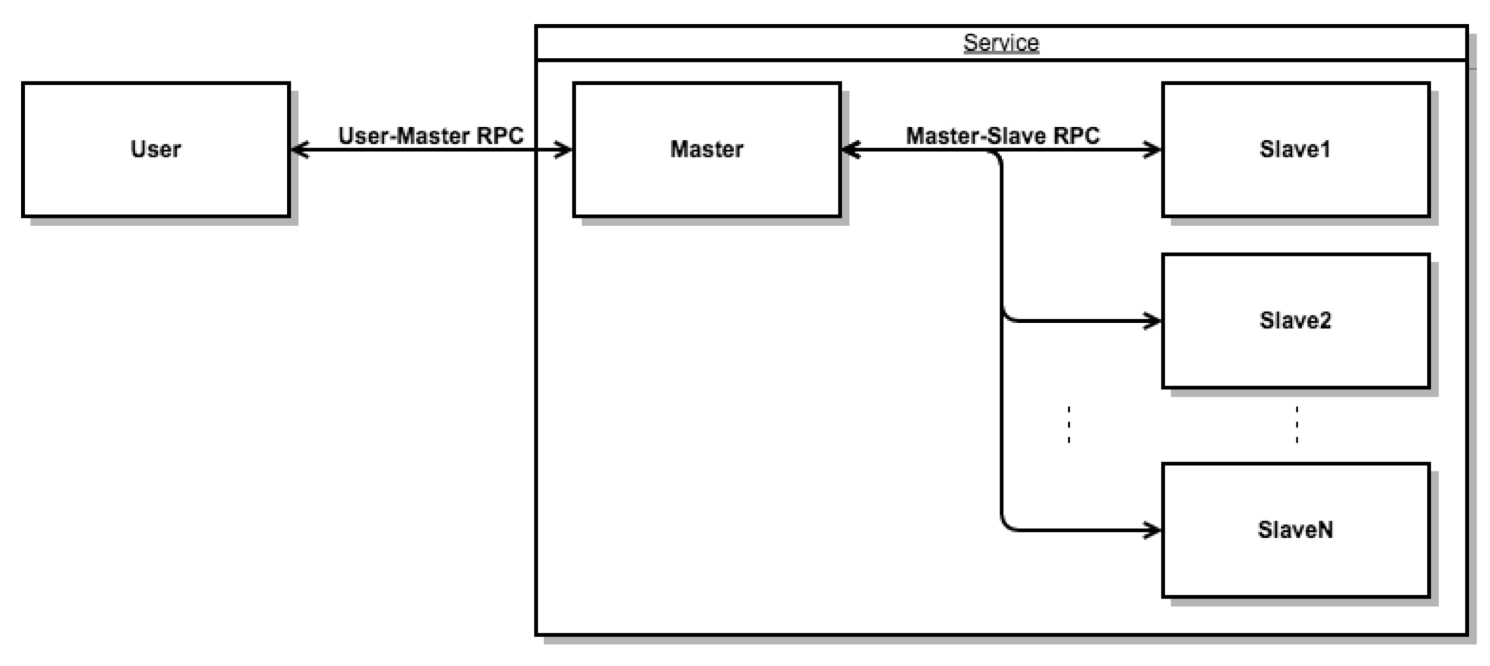
\includegraphics[width=0.9\textwidth]{img/component-diagram}
\caption{Component diagram for the distributed minimax service showing the separation of \emph{user}, \emph{master}, and \emph{slave} processes}
\label{fig:component-diagram}
\end{center}
\end{figure}

A single \emph{master} process and a number of identical \emph{slave} processes communicate with each other to provide a network \emph{service} to a \emph{user} process. As illustrated in Figure~\ref{fig:component-diagram}, the \emph{user} and the \emph{slaves} communicate only with the \emph{master} (over the \emph{User-Master RPC} and \emph{Master-Slave RPC}, respectively) and not with each other.

On receiving a request from the \emph{user} over the \emph{User-Master RPC}, the \emph{master} creates a \emph{job pool} by breaking down the Minimax algorithm into discrete jobs that can be performed concurrently, and distributes these jobs to the slaves over the \emph{Master-Slave RPC}. The \emph{slaves} execute their jobs and return the results of their analyses to the \emph{master}. The \emph{master} consolidates these results into a single \emph{best move} suggestion and returns this to the \emph{user}.


%
% Module-Level Descriptions
%
\subsection{Module-Level Descriptions}\label{sec:modules}

This section gives a formal description of the major modules referenced in the previous section. Each module's inputs and outputs are listed along with a brief description of the module's purpose. The final design of each module is also described, and areas for potential improvement are noted in some cases.

% User-Master RPC
\subsubsection{User-Master RPC}

\paragraph{Module Inputs:}
\begin{itemize}
\item Serialized game state
\item Time limit
\end{itemize}

\paragraph{Module Outputs:}
\begin{itemize}
\item Suggestion for best move
\end{itemize}

\paragraph{Module Description:\\}
This module represents network interaction between the \emph{user} and the \emph{master}.

The user makes a request to the master with a serialized game state and a maximum time allowed. The Master node is expected to confer with the slaves and respond within the time limit with its suggestion for a move to be played.

\paragraph{Final Design:\\}
The open-source \emph{Protobuf} library[4] was used to describe the message formats and generate RPC code. For an exact specification of the RPC, see Section~\ref{sec:protobuf-sample} in Appendix C.

% Job Pool Creation
\subsubsection{Job Pool Creation}

\paragraph{Module Inputs:}
\begin{itemize}
\item Game state to be analyzed
\item A set of slaves that are available to do work
\end{itemize}

\paragraph{Module Outputs:}
\begin{itemize}
\item A set of jobs that can be worked independently and concurrently
\end{itemize}

\paragraph{Module Description:\\}
This module is a component of the \emph{master}.

Given a game state, this module generates a set of jobs that can be worked independently. The number of jobs created will depend on the number of slaves available to do work. In particular, it should produce at least as many jobs as there are slaves, so no slave is left with no work to do.

\paragraph{Final Design:\\}
A \emph{job} in the final design is a game state that is a descendent\footnote{The "children" of a game state are the game states that can be reached by making a single move. For example, an empty tic-tac-toe board has nine children, representing a piece played in each of the nine empty spots. The "descendents" of a game state are its children, its children's children, etc.} of the game state to be analyzed. This module will examine the direct descendents of the viven game state, then each of their direct descendents, etc., until the number of descendents is greater than the number of slaves. When that condition is met, these game states are returned as jobs.


% Job Allocation
\subsubsection{Job Allocation}\label{sec:job-allocation}

\paragraph{Module Inputs:}
\begin{itemize}
\item A set of jobs that can be worked independently and concurrently
\item A set of \emph{slaves} that are available to do work
\end{itemize}

\paragraph{Module Outputs:}
\begin{itemize}
\item Exactly one \emph{slave} assigned to each job
\end{itemize}

\paragraph{Module Description:\\}
This module is a component of the \emph{master}.

Given a set of jobs and a set of \emph{slaves}, this module decides which \emph{slaves} will work on which jobs.

\paragraph{Final Design:\\}
The final design assigns jobs to slaves in a round-robin fashion. For example, if there are 10 jobs and 7 slaves, then the first three slaves will be assigned two jobs each, and the other four slaves will be assigned only one job. This method ensures that the \emph{number} of jobs assigned to each slave is fairly even, but is agnostic about \emph{which} jobs are assigned to which slave.

This is a major area for improvement. Given more time, this module should attempt to measure the relative importance of jobs and the effectiveness of slaves at performing work, and assign more important jobs to more effective slaves.

% Master-Slave RPC
\subsubsection{Master-Slave RPC}

\paragraph{Module Inputs:}
\begin{itemize}
\item A set of jobs
\item Time Limit
\end{itemize}

\paragraph{Module Outputs:}
\begin{itemize}
\item Result of analysis for each job
\end{itemize}

\paragraph{Module Description:\\}
This module represents network interaction between the \emph{master} and the \emph{slaves}.

The master delivers to each slave a set of jobs to be performed and a maximum time allowed. The slaves return their results to the Master within the allowed time.

This module deals primarily with serialization and communication with the master node, while the \emph{Slave Work} module below deals primarily with performing analysis.

\paragraph{Final Design:\\}
The open-source \emph{Protobuf} library[4] was used to describe the message formats and generate RPC code. For an exact specification of the RPC, see Section~\ref{sec:protobuf-sample} in Appendix C.


% Slave Work
\subsubsection{Slave Work}

\paragraph{Module Inputs:}
\begin{itemize}
\item A set of jobs
\item Time Limit
\end{itemize}

\paragraph{Module Outputs:}
\begin{itemize}
\item Result of analysis for each job
\end{itemize}

\paragraph{Module Description:\\}
This module is a component of the \emph{slaves}.

This module performs executes the jobs that were allocated by the master. This involves running the Minimax algorithm on subsets of the game tree. The results of the jobs are returned to the \emph{Master-Slave} RPC module to be returned to the master.

\paragraph{Final Design:\\}
This module receives a set of game states to analyze and a time limit, and produces a heuristic evaluation of each game state. For each game state, concurrently, it will run an iterative-deepening Minimax[5] algorithm\footnote{The Minimax algorithm is run first with a cut-off depth of 1, then 2, then 3, etc. until time runs out.}, analyzing to increasing depths until time runs out. When the time limit has elapsed, the results of the last complete iteration for each game state are returned.


% Result Consolidation
\subsubsection{Result Consolidation}

\paragraph{Module Inputs:}
\begin{itemize}
\item Results of analysis for each job
\end{itemize}

\paragraph{Module Outputs:}
\begin{itemize}
\item Suggestion for best move
\end{itemize}

\paragraph{Module Description:\\}
This module is a component of the \emph{master}.

This module combines the results of the analyses that the slaves performed to produce a single best move suggestion to return to the user.

\paragraph{Final Design:\\}
Given a set of game states that are descendents of the "parent" game state for which the user requested analysis, this module runs the Minimax algorithm rooted at the parent, using the slaves' heuristic evaluations. The output of this Minimax evaluation is returned to the user as the suggested best move.


%
% Testing and Verification
%
\section{Testing and Verification}

This section introduces a test for each requirement, constraint, and objective introduced in Section~\ref{sec:requirements}. The results of each test are included along with a short discussion concluding whether or not each requirement was met.

% Tests: Functional Requirements

\subsection{\textbf{Requirement:} \emph{shall correctly implement the minimax algorithm}}\label{sec:req-correctness}

\subsection{\textbf{Requirement:} \emph{allow for distribution over a number of nodes between 2 and 10}}

% Test
\subsubsection{\textbf{Test:} Two-Node Cluster}

\paragraph{Test description:} Analyze a Connect-4 game state using a cluster of 2 slaves

\paragraph{Pass Criteria:} The analysis completes without error, and the result of the analysis is an optimal move.

\paragraph{Test Result:} PASS

Included here is the raw log output from the user process (Figure~\ref{fig:duo-user-3}) and the master process (Figure~\ref{fig:duo-master-3}) when this test was run. 

\begin{figure}[h]
\lstinputlisting[firstline=2]{../aws/logs/duo-user-3.log}
\caption{The raw output of the user process with a 2-node slave cluster}
\label{fig:duo-user-3}
\end{figure}

\begin{figure}[h]
\lstinputlisting[firstline=2,lastline=11]{../aws/logs/duo-master-3.log}
\caption{The first 10 lines of raw output of the master process with a 2-slave cluster. The complete log is too long to list here.}
\label{fig:duo-master-3}
\end{figure}

We can verify that this is a 2-slave cluster in line 8 of Figure~\ref{fig:duo-master-3}. We can further verify that the analsyis completed without error and that the result of the analysis (at the bottom of Figure~\ref{fig:duo-user-3} was an optimal move\footnote{The rules of Connect-4 are not included in this document, but are widely available. In this case, the recommended move is optimal because any other move would lead to an immediate win by X playing in the same spot.}. Since the analysis completed successfully and without error for a cluster of 2 slaves, this test is considered to have passed.

% Test
\subsubsection{\textbf{Test:} Ten-Node Cluster}

\paragraph{Test description:} Analyze a Connect-4 game state using a cluster of 10 slaves

\paragraph{Pass Criteria:} The analysis completes without error, and the result of the analysis is an optimal move.

\paragraph{Test Result:} PASS

A cluster of 10 slaves was used to analyze the same Connect-4 state, and the same (optimal) result was returned. Relevant lines of the master process's log output are shown in Figure~\ref{fig:master-3}.

\begin{figure}[h]
\lstinputlisting[firstline=1,lastline=4]{../aws/logs/master-3.log}
\caption{An excerpt of the raw output of the master process with a 10-slave cluster. The complete log is too long to list here.}
\label{fig:master-3}
\end{figure}

It can be seen in this log output that 10 slaves are used. Since the analysis completed successfully and without error using a cluster of 10 slaves, this test is considered to have passed.

% Test
\subsection{\textbf{Requirement:} \emph{allow the user to set a time limit on the computation; enforce within 0.5 seconds}}

\subsubsection{\textbf{Test:} Time limit of 3 seconds}

\paragraph{Test description:} Analyze a Connect-4 game state using an imposed time limit of 3 seconds. 

\paragraph{Pass Criteria:} The result is returned in at most 3.5 seconds.

\paragraph{Test Result:} PASS

Figure~\ref{fig:duo-user-3} shows the output of the user process when this test was run. Line 9 shows that the request was made with a limit of 3 seconds, and line 10 shows that the response was returned in 3.18 seconds. Since the time limit was enforced within 0.5 seconds, this test is considered to have passed.

% Test
\subsubsection{\textbf{Test:} Time limit of 10 seconds}

\paragraph{Test description:} Analyze a Connect-4 game state using an imposed time limit of 10 seconds. 

\paragraph{Pass Criteria:} The result is returned in at most 10.5 seconds.

\paragraph{Test Result:} PASS

Figure~\ref{fig:user-10} shows the output of the user process when this test was run. Line 9 shows that the request was made with a limit of 10 seconds, and line 10 shows that the response was returned in 10.16 seconds. Since the time limit was enforced within 0.5 seconds, this test is considered to have passed.

\begin{figure}[h]
\lstinputlisting[firstline=2]{../aws/logs/user-10.log}
\caption{The output of the user process with a specified time limit of 10 seconds.}
\label{fig:user-10}
\end{figure}


% Tests: Constraints

\subsection{\textbf{Constraint:} \emph{must be executable on Mac OS 10.9, Windows 8.1, and Linux 3.14}}

% Test
\subsubsection{\textbf{Test:} Windows 8.1}

\paragraph{Test Description:} Analyze a game state with all master and slave processes running on Windows 8.1.

\paragraph{Pass Criteria:} The analysis completes without error.

\paragraph{Test Result:} PASS

Figure~\ref{fig:win8} in Appendix D is a screenshot of a master, a user, and two slave processes running successfully in a Windows 8.1 environment.

% Test
\subsubsection{\textbf{Test:} Mac OS 10.9}

\paragraph{Test Description:} Analyze a game state with all master and slave processes running on Mac OS 9.

\paragraph{Pass Criteria:} The analysis completes without error.

\paragraph{Test Result:} PASS

Figure~\ref{fig:osx} in Appendix D is a screenshot of a master, a user, and two slave processes running successfully in a Mac OS 10.9 environment.

% Test
\subsubsection{\textbf{Test:} Linux 3.14}

\paragraph{Test Description:} Analyze a game state with all master and slave processes running on Linux 3.14.

\paragraph{Pass Criteria:} The analysis completes without error.

\paragraph{Test Result:} PASS

Figure~\ref{fig:linux} in Appendix D is a screenshot of a master, a user, and a slave process running successfully on an Amazon Linux AMI[6] using kernel version 3.14.


% Tests: Objectives

\subsection{\textbf{Objective:} \emph{evaluate more game states than the non-distributed implementation}}\label{sec:obj-number-analyzed}

% Test
\subsubsection{\textbf{Test:} Distributed vs. Non-Distributed}\label{sec:number-analyzed}

\paragraph{Test description:} Analyze the same Connect-4 state using (1) a cluster of 10 slaves, and (2) a single computer. Ensure that the single computer is given the same processing time as the cluster took for communication, coordination, and processing combined. Measure the number of game states analyzed during the computations.

\paragraph{Pass Criteria:} The cluster of 10 slaves analyzes more game states than the single computer.

\paragraph{Test Result:} PASS

The number of states analyzed was measured for four analyses: with 10 slaves, given 3 seconds and given 10 seconds, and with 1 slave given the same time constraints. The results are shown in Figure~\ref{fig:number-analyzed}.

\begin{figure}[h]
\begin{center}
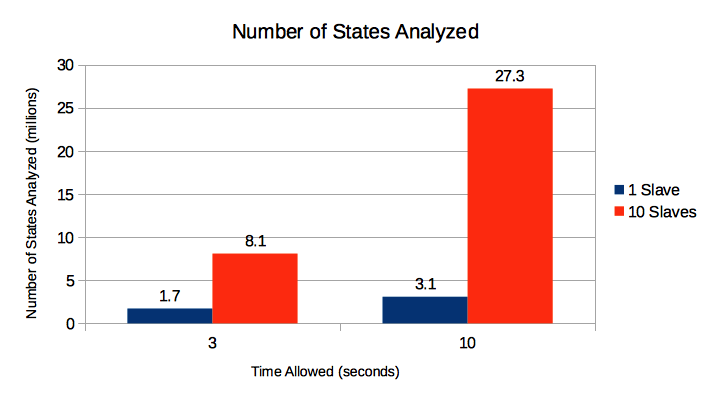
\includegraphics[width=0.9\textwidth]{img/number-analyzed}
\caption{The number of states analyzed by two slave clusters (one with a single computer, the other with 10 slaves) given 3 seconds and 10 seconds}
\label{fig:number-analyzed}
\end{center}
\end{figure}

Note that for both time limits, the cluster of 10 slaves analyzed more states than the single computer. For this reason, this test is considered to have passed, and the objective met. 

\subsection{\textbf{Objective:} \emph{should maximize throughput on different combinations of fast and slow processors}}

% Test
\subsubsection{\textbf{Test:} Analyze different combinations of fast and slow CPUs}

\paragraph{Test Description:} See Section 3.6 of Appendix B for a description of the originally-proposed test.

\paragraph{Test Result:} FAIL

The work required for this test to pass was not completed, and the test was abandoned and assumed to fail. In particular, as mentioned in the "Final Design" paragraph of Section~\ref{sec:job-allocation}, the master's job allocation algorithm is only a simple round-robin assignment, agnostic to the processing capabilities of the different slaves. Given more time, this is a potential area for improvement of this project.

%
% Conclusions
%
\section{Summary and Conclusions}

The overarching purpose of this project was to provide a method to speed up the Minimax algorithm by making use of all available computing power. A user with many computers at his disposal should easily be able to coordinate them to work together on the Minimax problem, and provide better results than he would otherwise achieve with only a single computer.

The first functional requirement presented in Section~\ref{sec:requirements} ensures that the Minimax algorithm is implemented correctly, without which any improvements to execution speed would be worthless. This requirement was met, as demonstrated in Section~\ref{sec:req-correctness}.

The second requirement ensures that the number of computers is variable, i.e. that the system can will work successfully with different cluster sizes\footnote{Though the original project proposal required that the system work with up to 50 computers, this was reduced to 10 to make testing cheaper and easier. This change is not evidence that the system would \emph{not} work with 50 computers (in fact, due to the encouraging results seen in Section~\ref{sec:number-analyzed}, we predict that the system would work quite well with clusters of this size, and would like to test this prediction in the future).}. This requirement was also met by demonstrating that the same evaluation worked with a cluster of 2 slaves and a cluster of 10 slaves.

The third requirement ensures that the user can vary the amount of time available to do work. The framework produced for this project is written in a general, extensible way that would easily allow developers to run the Minimax algorithm on a wide variety of game-theoretic scenarios. Considering the range of possible applications, this requirement was added to ensure that the resulting framework is not overly restrictive in its scope. For similar reasons, the sole constraint in Section~\ref{sec:constraints} (that the software should be executable on a range of operating systems) was added as well. Both requirements were met.

However, as stated at the beginning of this section, the utility of this project is tied to its ability to provide \emph{better} results on a cluster of computers than it could otherwise achieve. If the overhead of network communication and coordination inherent in a distributed system makes cluster perform worse than a single computer, then this project -- while meeting requirements -- is not useful. This primary objective is laid out in Section~\ref{sec:objectives} and tested in Section~\ref{sec:number-analyzed}. The results, summarized in Figure~\ref{fig:number-analyzed} in that section, demonstrate that this objetive was met -- for two different time limits, the cluster of 10 slaves analyzed significantly more game states than a single computer running the Minimax algorithm.

Since the requirements and constraints were met, and this primary "usability" objective was achieved, we consider this project a success. 

A second objective was included Section~\ref{sec:objectives} addressing users who might have heterogeneous clusters. Ideally, the software should recognize differences in processing power between different computers in the cluster, and assign more work to more powerful computers. Work to this end was not completed by the time this report was writte, and so this objective is left unmet. A complete re-design of the job allocation module (Section~\ref{sec:job-allocation}) in pursuit of this objective would likely be the starting point for future work on this project.

%
% References
%
\pagebreak
\section{References}

[1] Russell, S., Norvig, P. \& Davis, E. (2010). Artificial intelligence: a modern approach. Upper Saddle River, NJ: Prentice Hall. (p. 122)

[2] Russell, S., Norvig, P. \& Davis, E. (2010). Artificial intelligence: a modern approach. Upper Saddle River, NJ: Prentice Hall. (p. 142)

[3] Steinerberger, S. (2014). On the number of positions in chess without promotion. International Journal of Game Theory.

[4] Google (2008). Protocol Buffers - Google's data interchange format.\\ \texttt{https://github.com/google/protobuf }

[5] Chess Programming Wiki (2015). Iterative Deepening.\\ \texttt{https://chessprogramming.wikispaces.com/Iterative+Deepening}

[6] Amazon (2015). Amazon Linux AMI.\\ \texttt{http://aws.amazon.com/amazon-linux-ami/}


%
% Appendix A: Gantt Chart History
%
\pagebreak
\section{Appendix A: Gantt Chart History}

This appendix includes the Gantt charts from the Project Proposal, the Test Document, and the Progress Report, as well as an updated Gantt chart which includes the work completed up to the day this report was submitted.

\begin{figure}[H]
\begin{center}
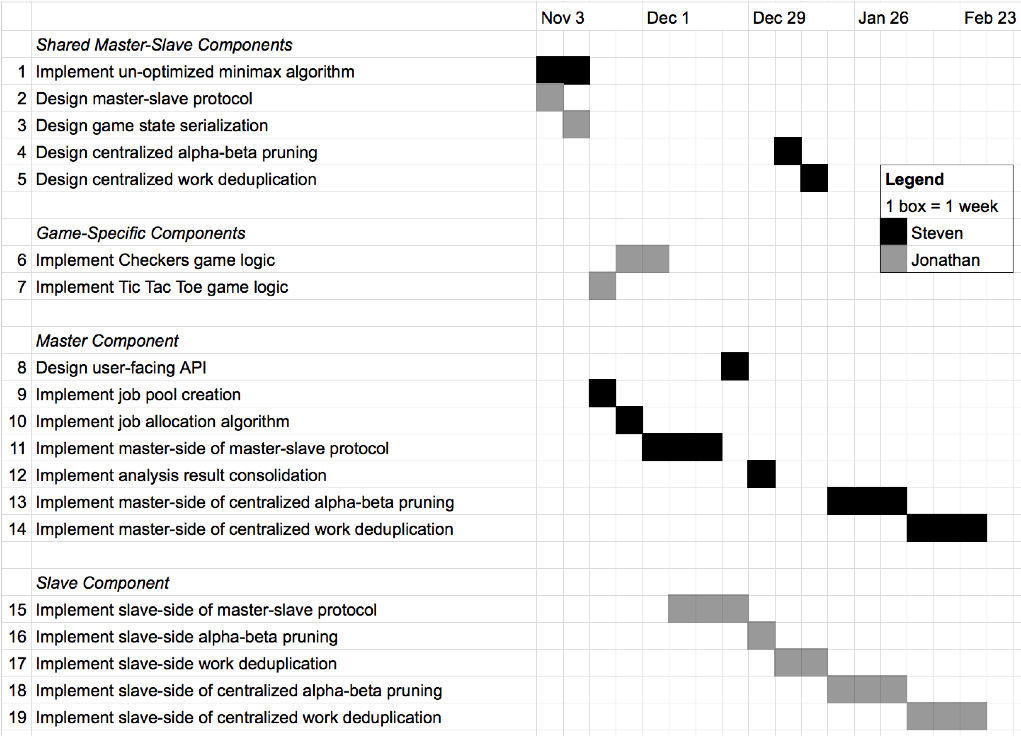
\includegraphics[width=0.9\textwidth]{img/gantt-proposal}
\caption{The initial Gantt chart, as presented in the Project Proposal.}
\end{center}
\end{figure}

\begin{figure}[H]
\begin{center}
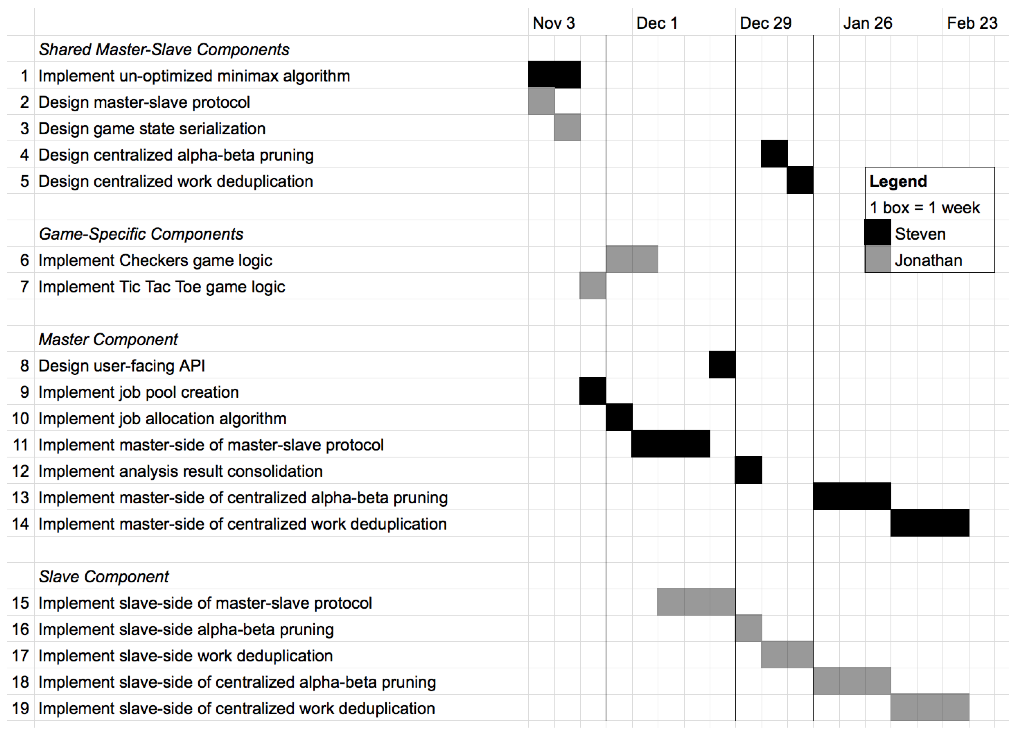
\includegraphics[width=0.9\textwidth]{img/gantt-test}
\caption{The Gantt chart from the Test Document}
\end{center}
\end{figure}

\begin{figure}[H]
\begin{center}
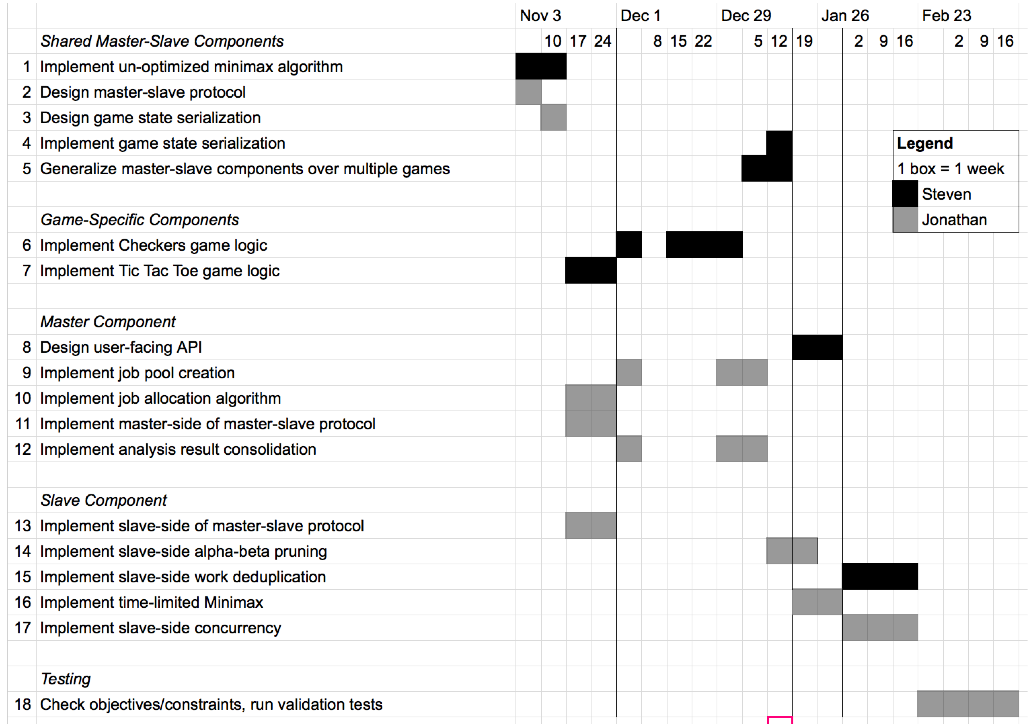
\includegraphics[width=0.9\textwidth]{img/gantt-progress}
\caption{The Gantt chart from the Progress Report}
\end{center}
\end{figure}

\begin{figure}[H]
\begin{center}
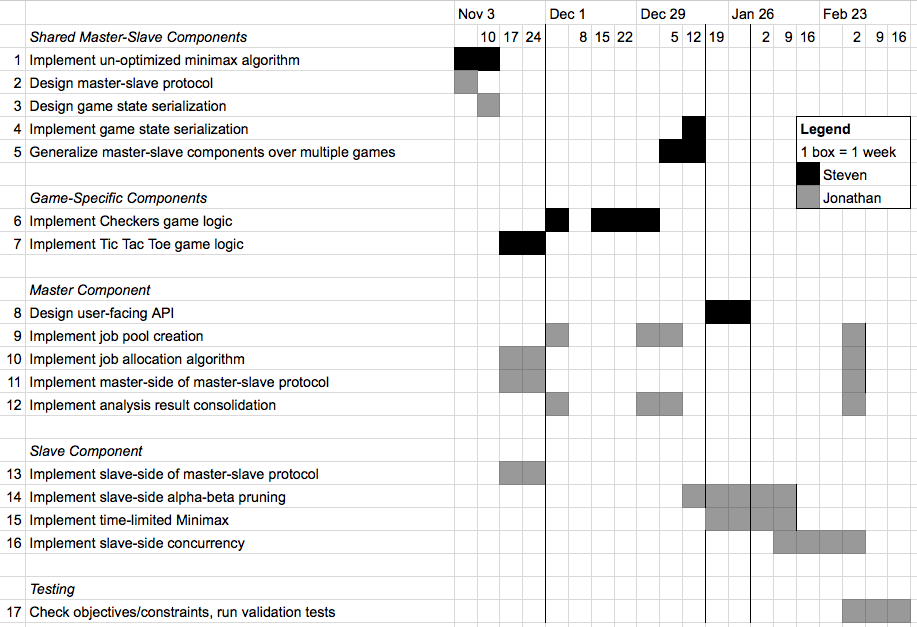
\includegraphics[width=0.9\textwidth]{img/gantt-final}
\caption{The final Gantt chart, representative of work done to this day.}
\end{center}
\end{figure}

%
% Appendix B: Original Validation and Acceptance Tests
%
\pagebreak
\includepdf[scale=0.8,pages={-},pagecommand=\section{Appendix B: Original Validation and Acceptance Tests}]{img/original-tests-1.pdf}
\includepdf[scale=0.8,pages={-}]{img/original-tests-2.pdf}
\includepdf[scale=0.8,pages={-}]{img/original-tests-3.pdf}


%
% Appendix C: Code Samples
%
\pagebreak
\section{Appendix C: Code Samples}

This appendix includes raw samples of code from the project to serve as further information for interested developers, and as proof of work for ECE496 administrators.

\subsection{Protobuf Specifications}\label{sec:protobuf-sample}

\subsubsection*{User-Master RPC}
\begin{lstlisting}
message DoWorkRequest {
    required bytes state = 1;
    required uint64 timeLimitMillis = 2;
}

message DoWorkResponse {
    required bytes move = 1;  // suggestion for next state
}

service UserService {
    rpc DoWork(DoWorkRequest) returns (DoWorkResponse);
}
\end{lstlisting}

\subsubsection*{Master-Slave RPC}
\begin{lstlisting}
message GetWorkRequest {
    message Result {
        required bytes state = 1;
        required int32 value = 2;  // should match Value type in game/game.go
        required int64 numStatesAnalyzed = 3;
    }
    // optionally return the results of a previous workload
    repeated Result result = 1;
}

message GetWorkResponse {
    repeated bytes state = 1;
    required uint64 timeLimitMillis = 2;
}

service SlaveService {
    rpc GetWork(GetWorkRequest) returns (GetWorkResponse);
}
\end{lstlisting}

%
% Appendix D: Screenshots
%
\pagebreak
\section{Appendix D: Screenshots}

This appendix includes screenshots taken during testing to serve as proof of work.

\begin{figure}[h]
\begin{center}
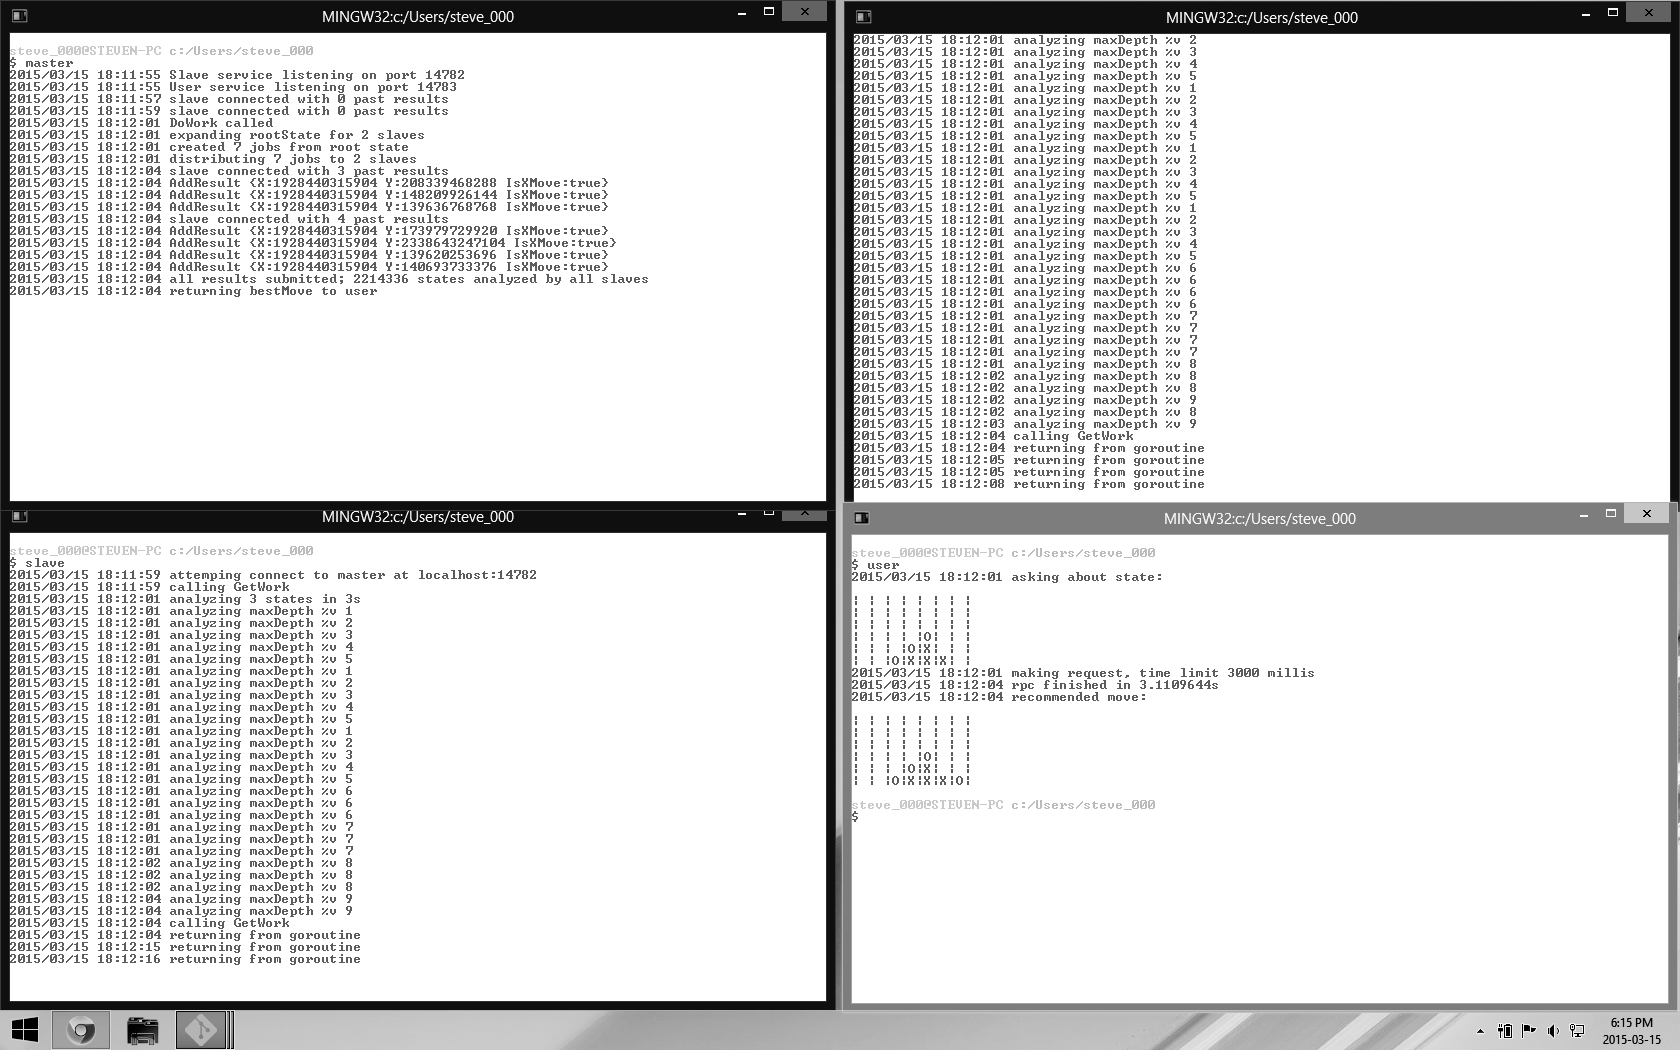
\includegraphics[width=0.7\textwidth]{img/win8}
\caption{A screenshot taken in a Windows 8.1 environment showing one master, one user, and two slave processes running successfully. Note that the colours have been modified to save ink if this document is printed.}
\label{fig:win8}
\end{center}
\end{figure}

\begin{figure}[h]
\begin{center}
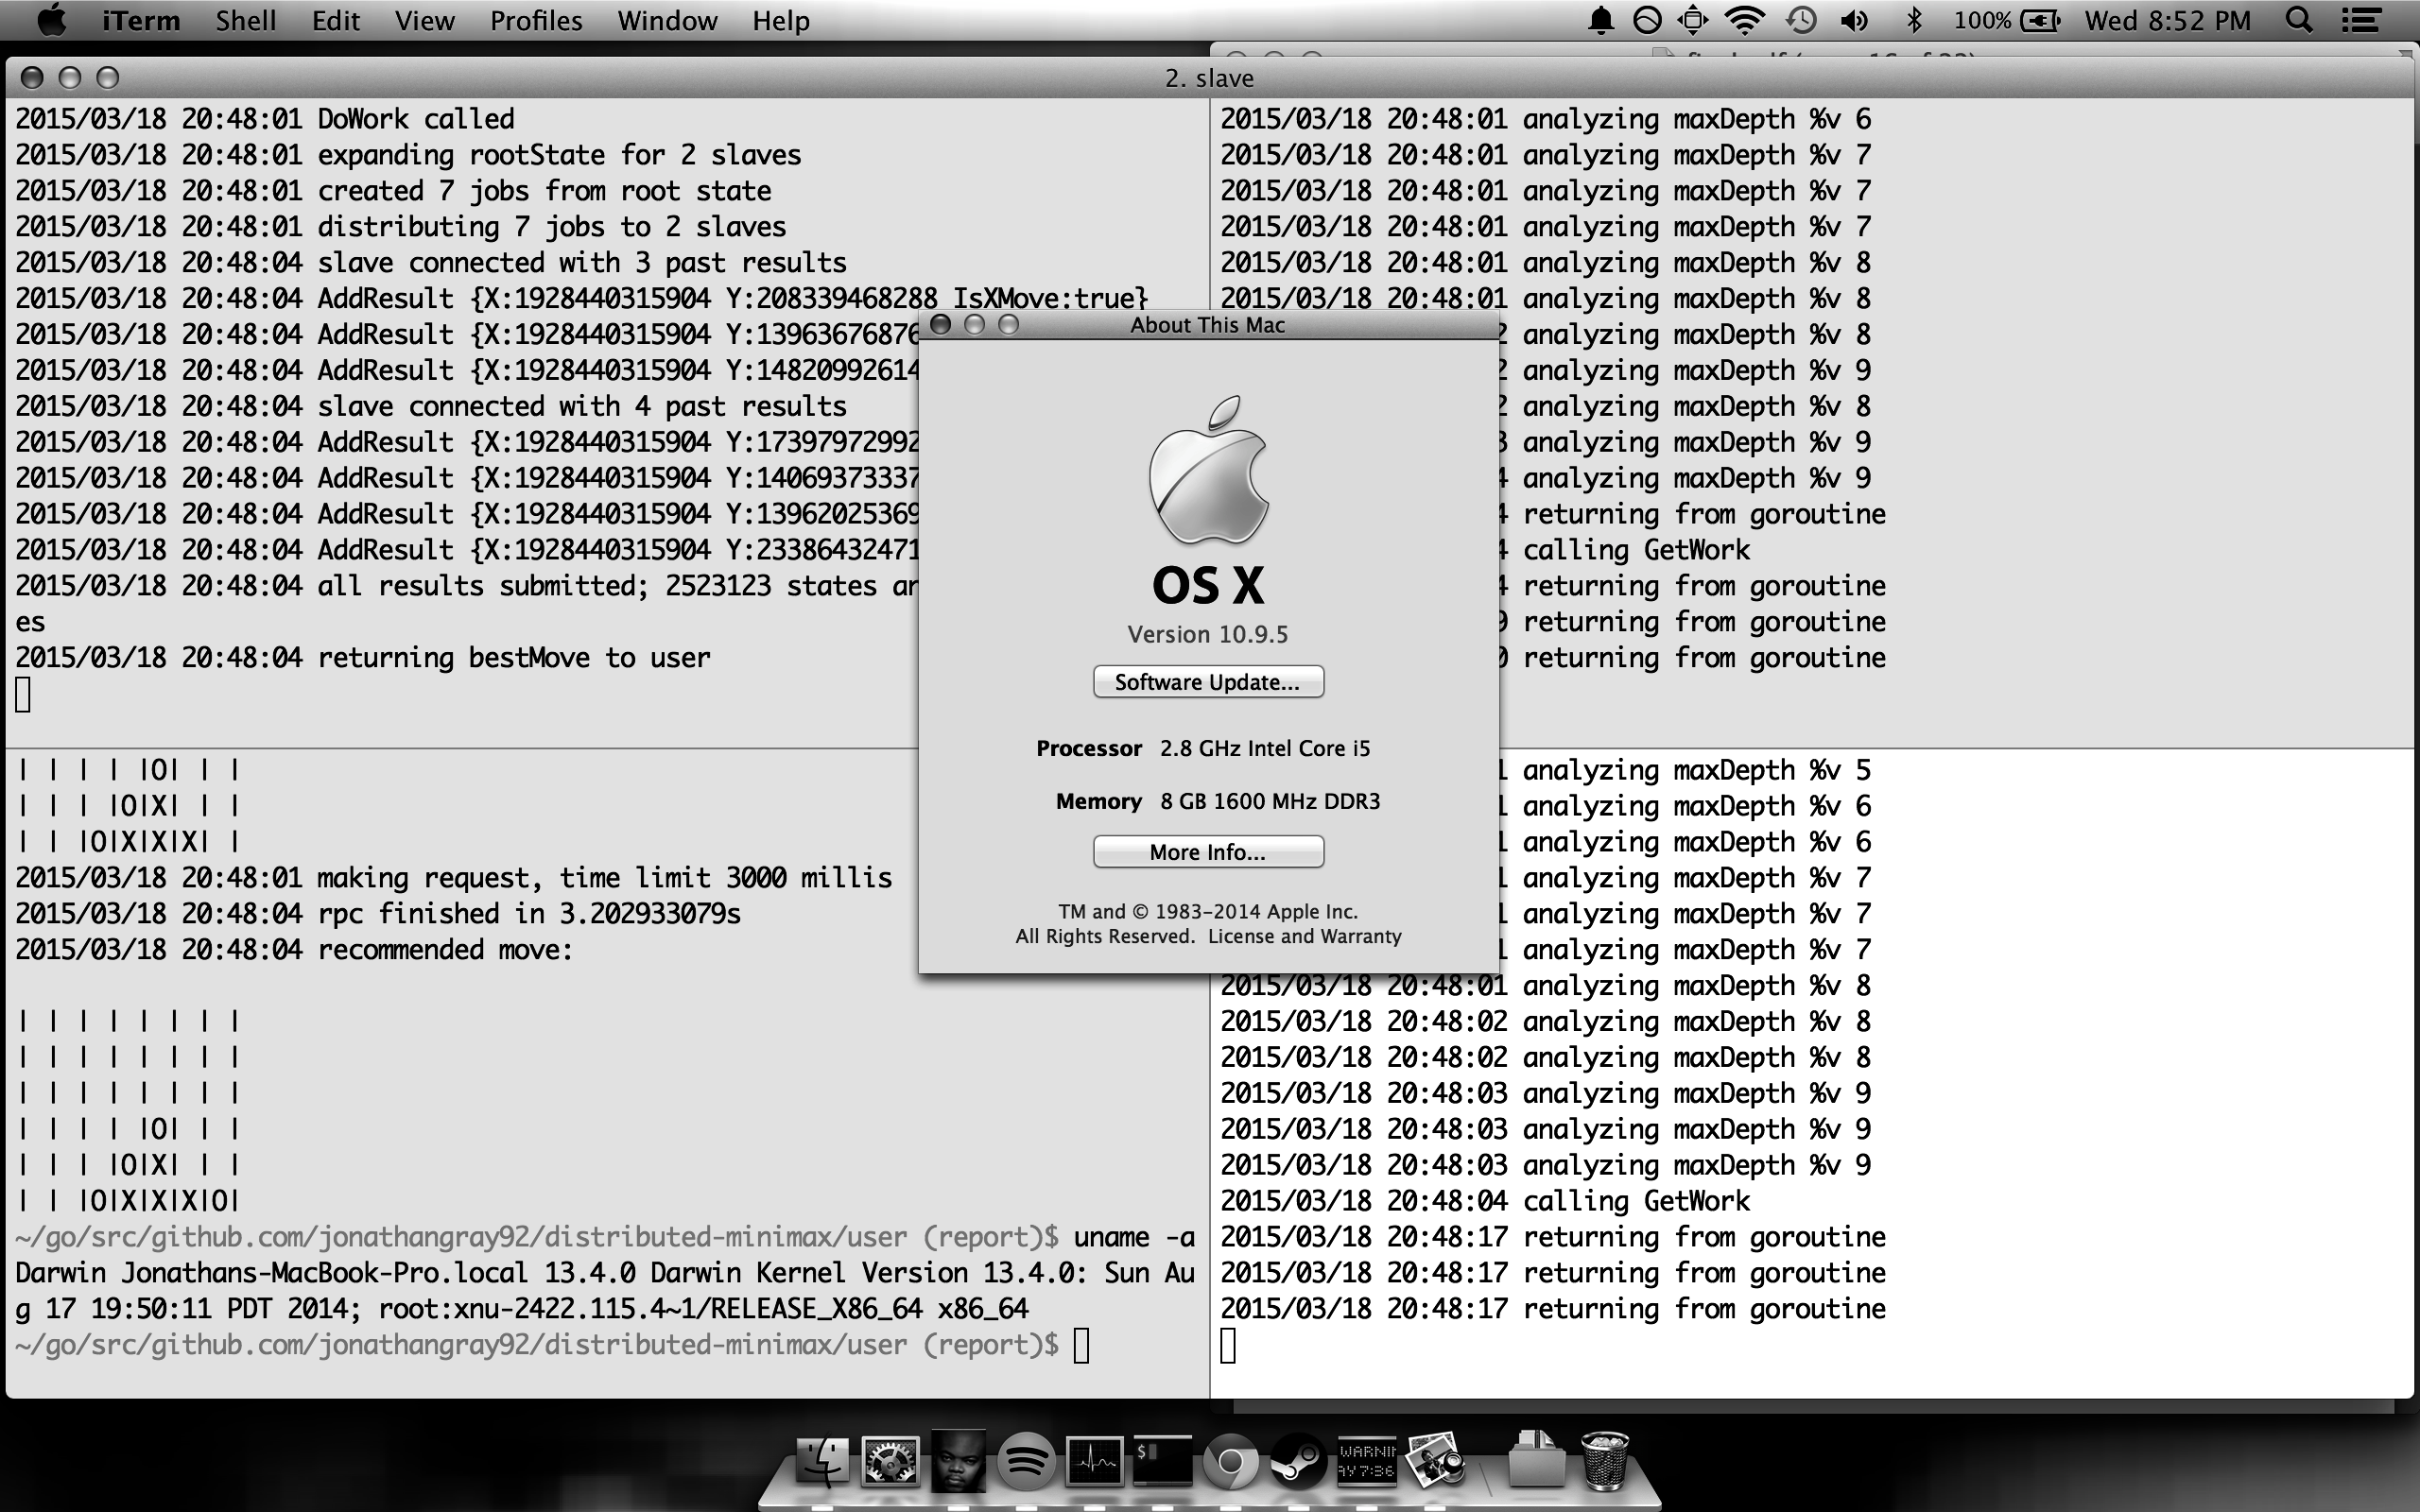
\includegraphics[width=0.7\textwidth]{img/osx}
\caption{A screenshot taken in an OS 10.9 environment showing one master, one user, and two slave processes running successfully. Note that the colours have been modified to save ink if this document is printed.}
\label{fig:osx}
\end{center}
\end{figure}

\begin{figure}[h]
\begin{center}
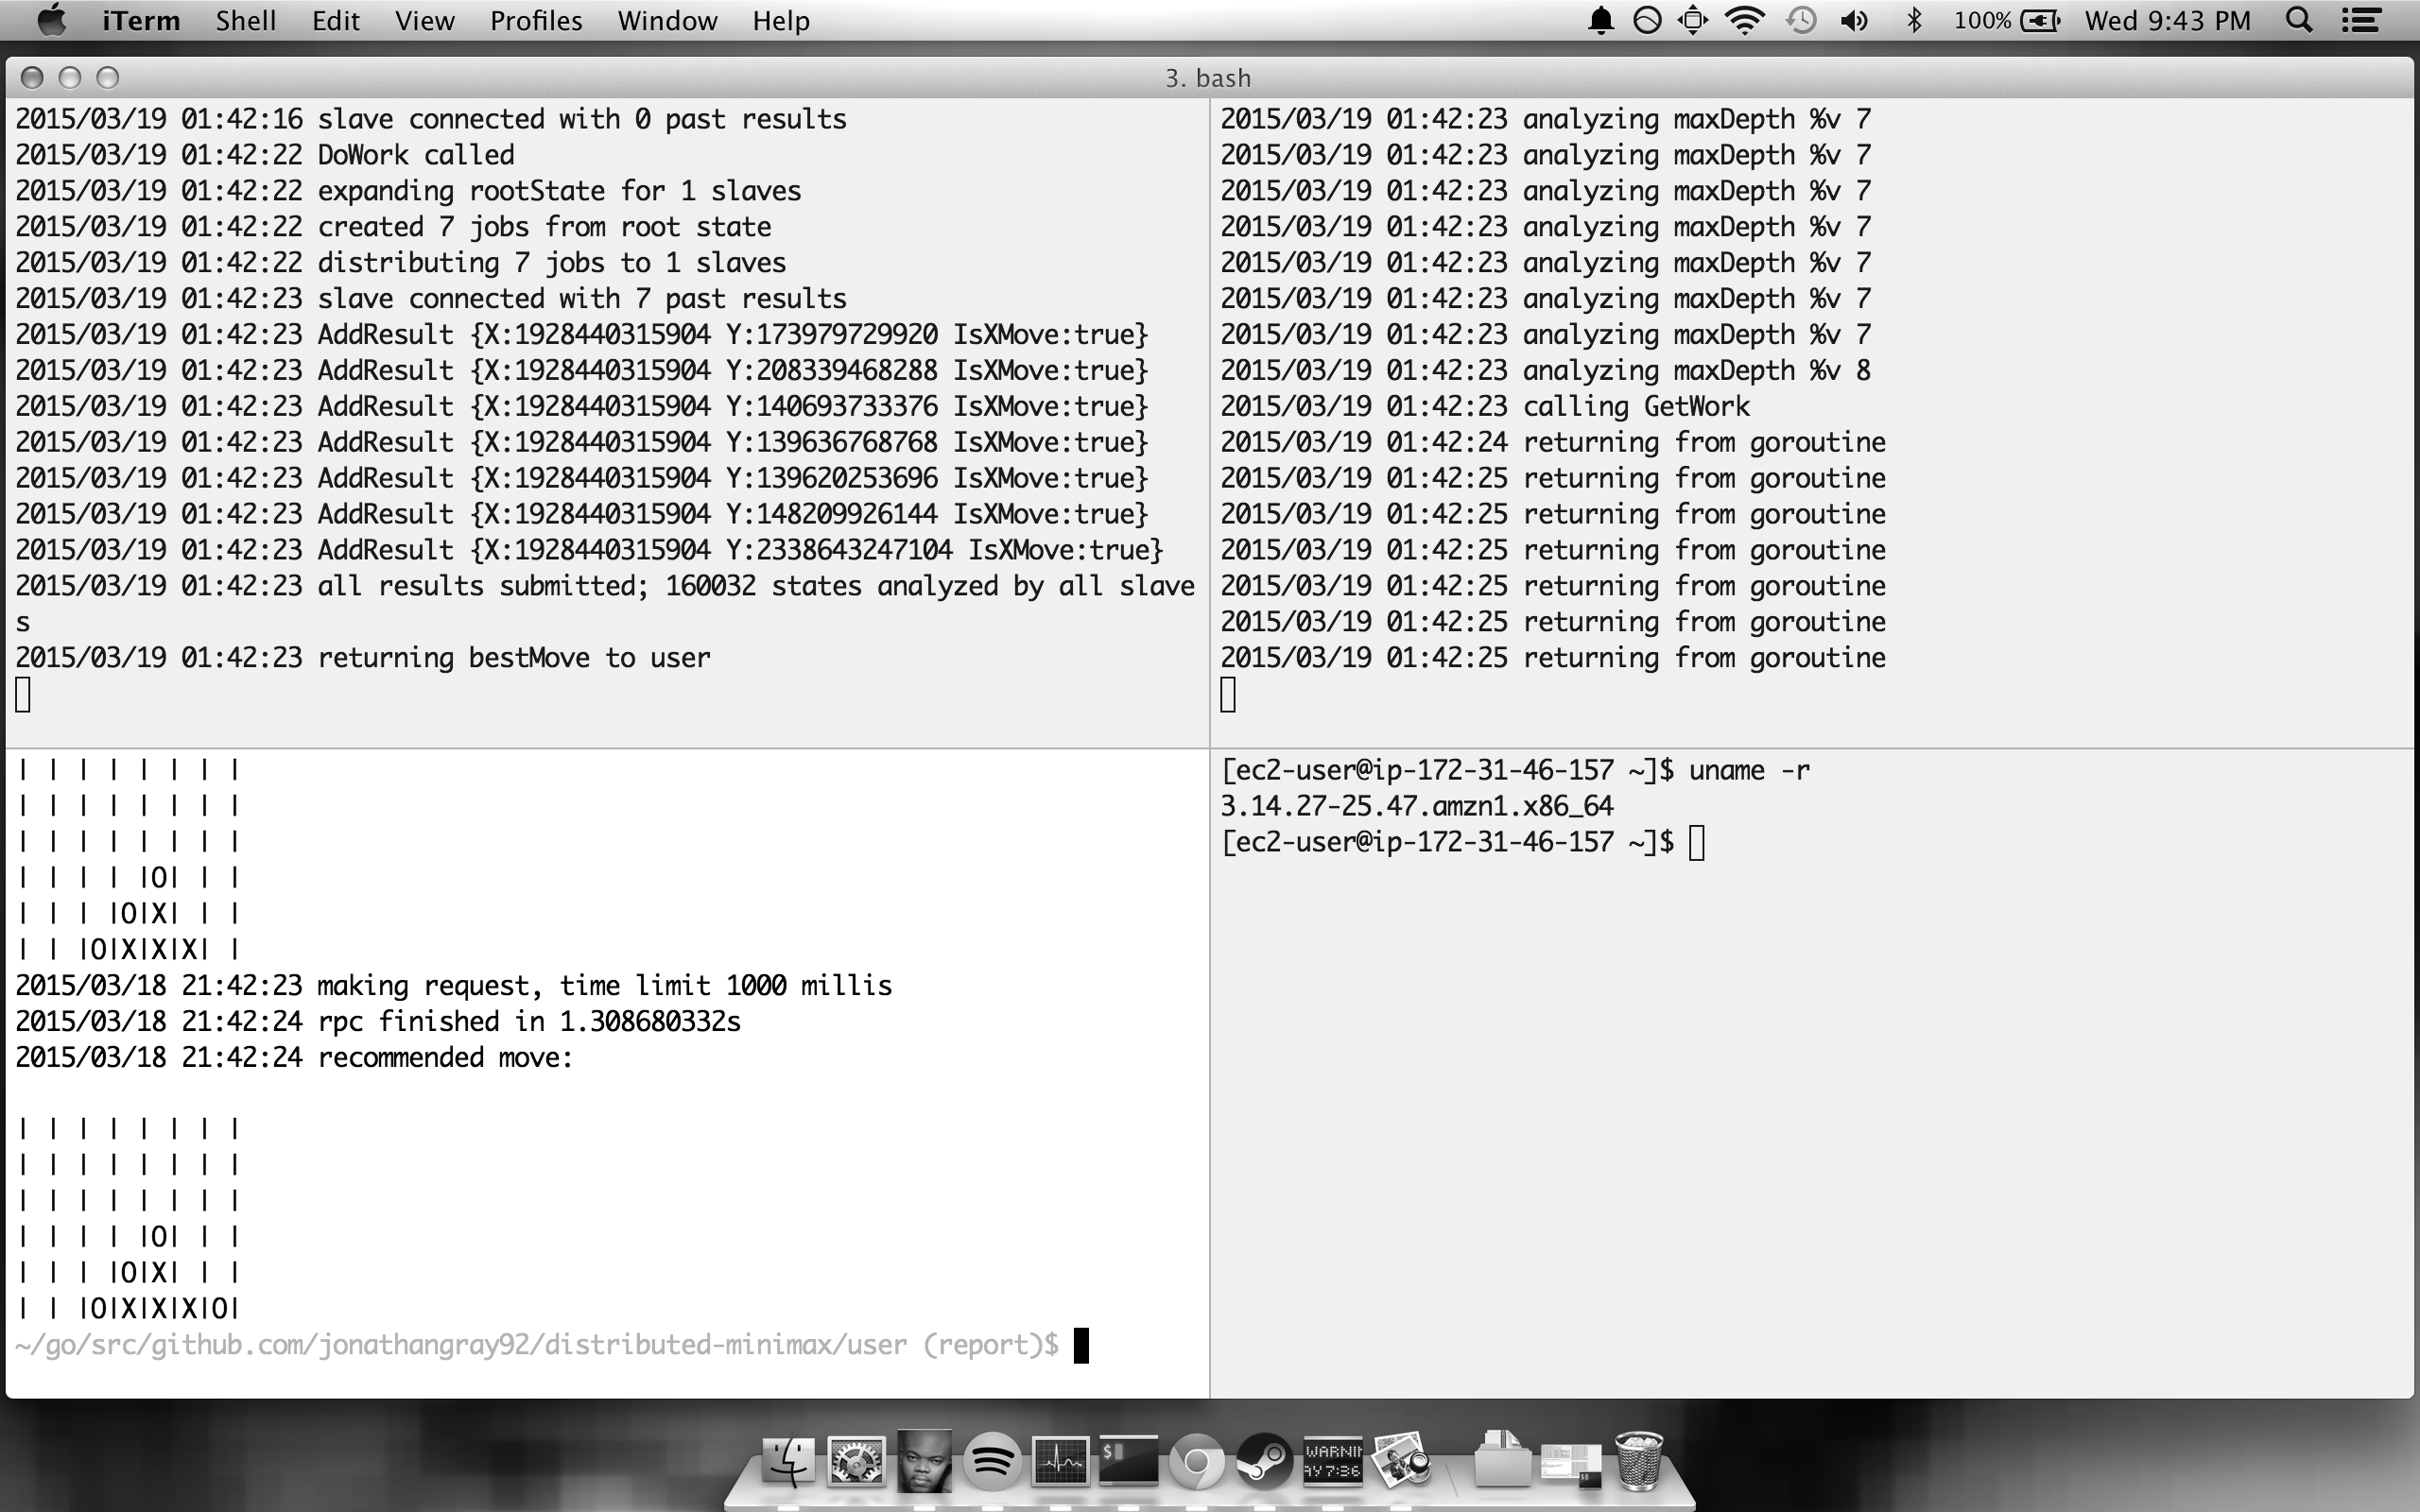
\includegraphics[width=0.7\textwidth]{img/linux}
\caption{A screenshot taken in an Amazon Linux AMI environment showing one master, one user, and one slave process running successfully. Note that the Linux kernel version is printed in the bottom-right, and is 3.14.}
\label{fig:linux}
\end{center}
\end{figure}

\end{document}
